\newpage

\section*{ $^{24}$Mg(n,p)$^{24}$Na }

Power Level: 100 kW(th) \\
Time at Power: 60.0 s \\
Wait Time:  2.0 h \\
Counting Time: 60.0 m \\
Total Activity at Removal: 6.98e-04 $\mu Ci$

\begin{table*}[h]
\centering
\begin{tabular}{ |c|c|c|c|c|c| }
 \hline
 Position & Mass $mg$ & Counting Activity $\mu Ci$ & Area (Counts) & Error \% \\
 \hline 
 1 & 0.26 & 1.46e-04 & 2.85e+02 & 5.9265 \\ 
\hline
 2 & 0.26 & 2.17e-04 & 4.25e+02 & 4.8532 \\ 
\hline
 3 & 0.26 & 1.67e-04 & 3.27e+02 & 5.5314 \\ 
\hline
 4 & 0.26 & 7.42e-05 & 1.45e+02 & 8.3081 \\ 
\hline
\end{tabular}
\end{table*}

\begin{figure}[h]
\centering
\begin{subfigure}{.5\textwidth}
  \centering
     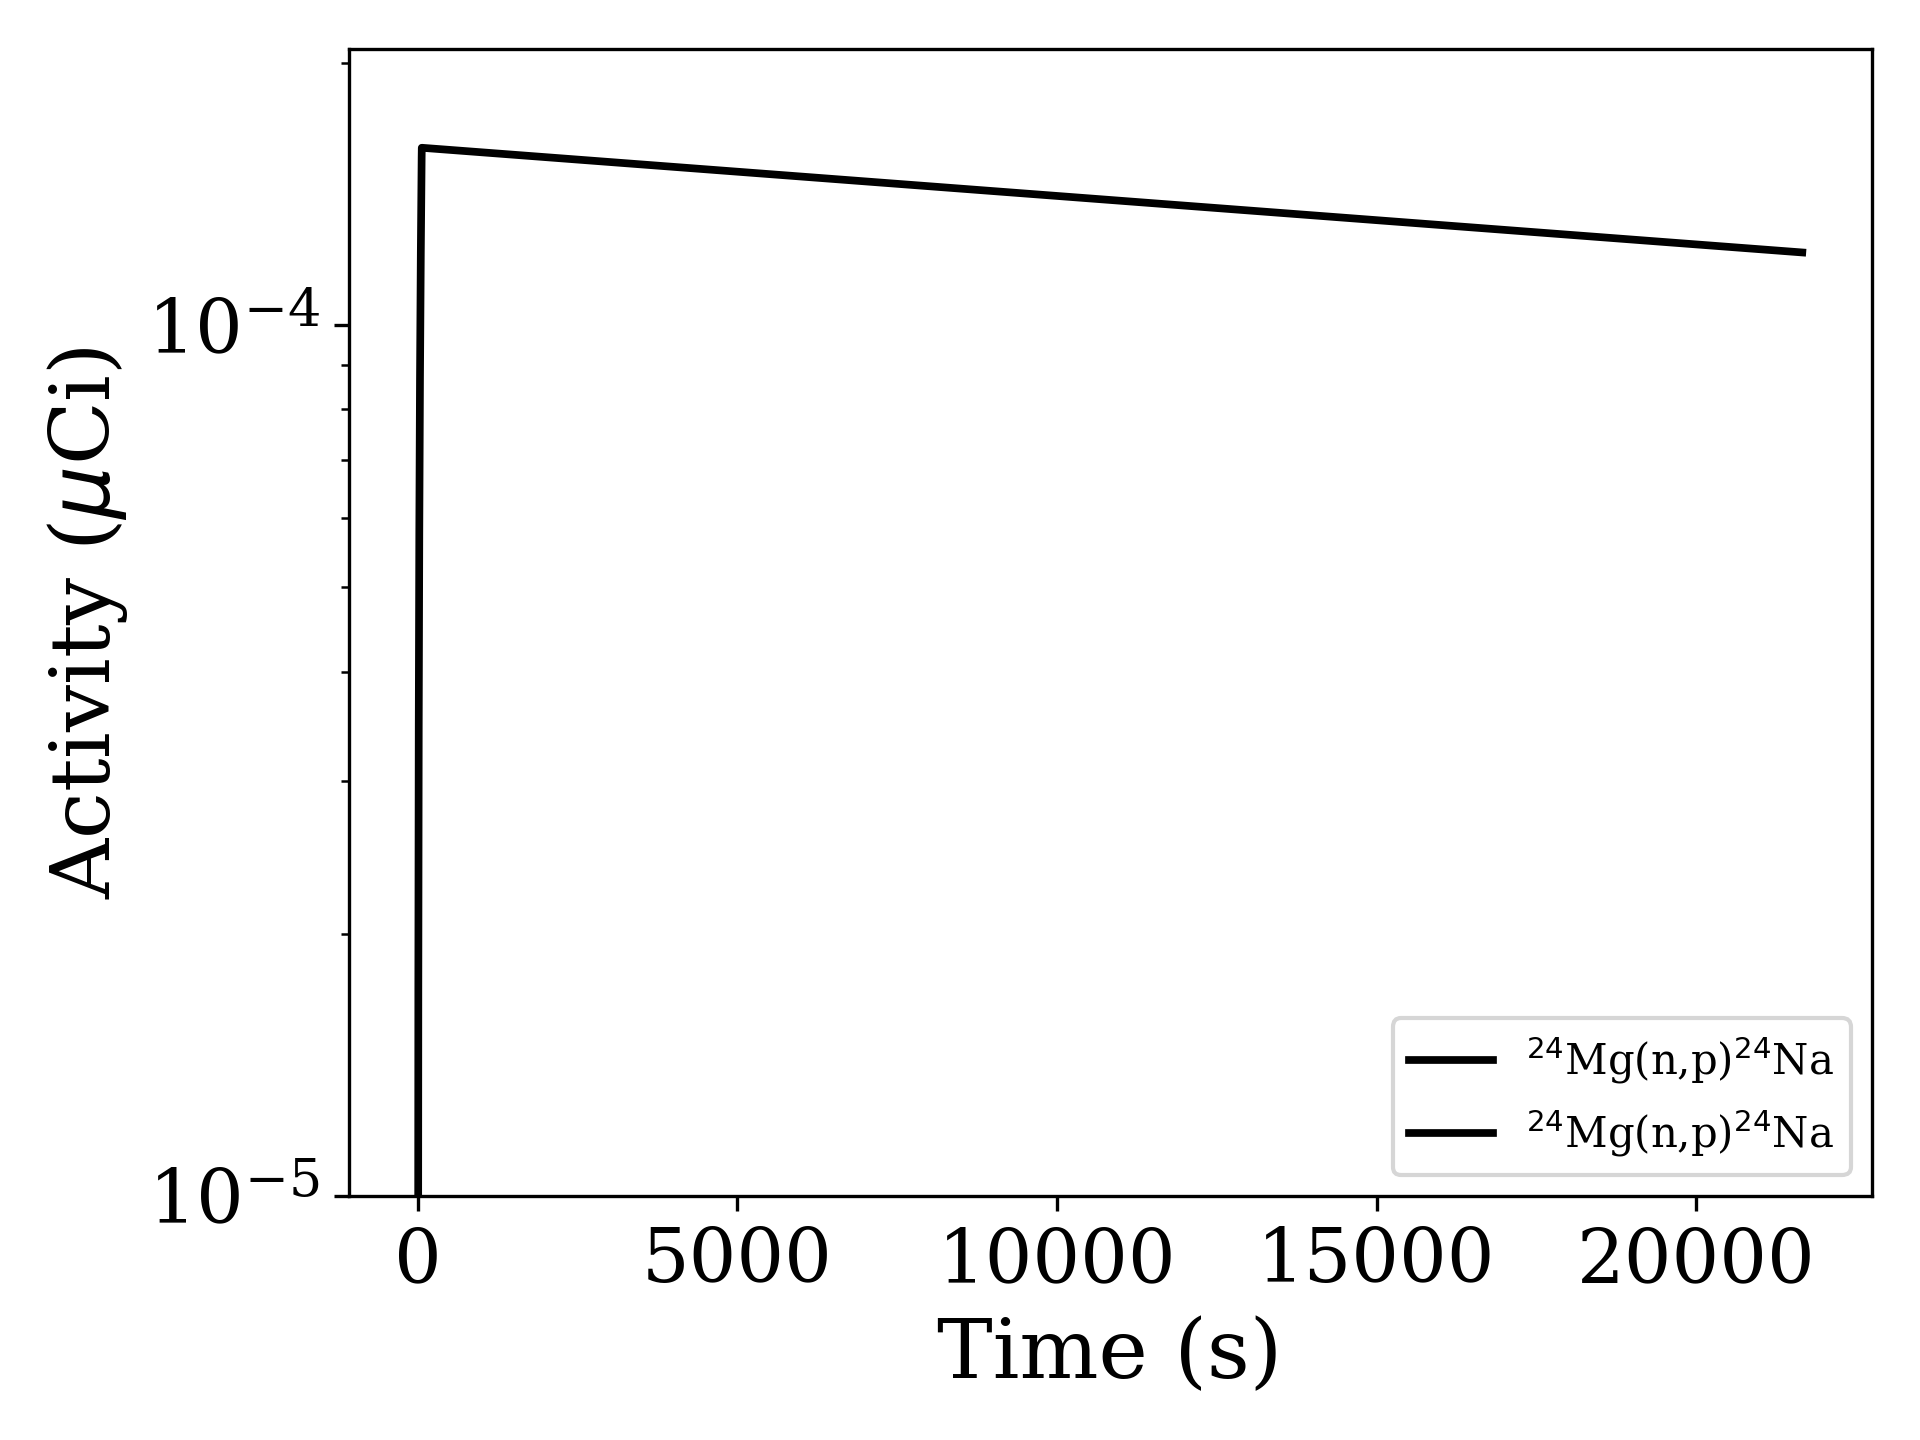
\includegraphics[width=.8\textwidth]{plot/Mg-24(n,p)Na-24_library1} 

  \caption{A subfigure}
  \label{fig:sub1}
\end{subfigure}%
\begin{subfigure}{.5\textwidth}
  \centering
     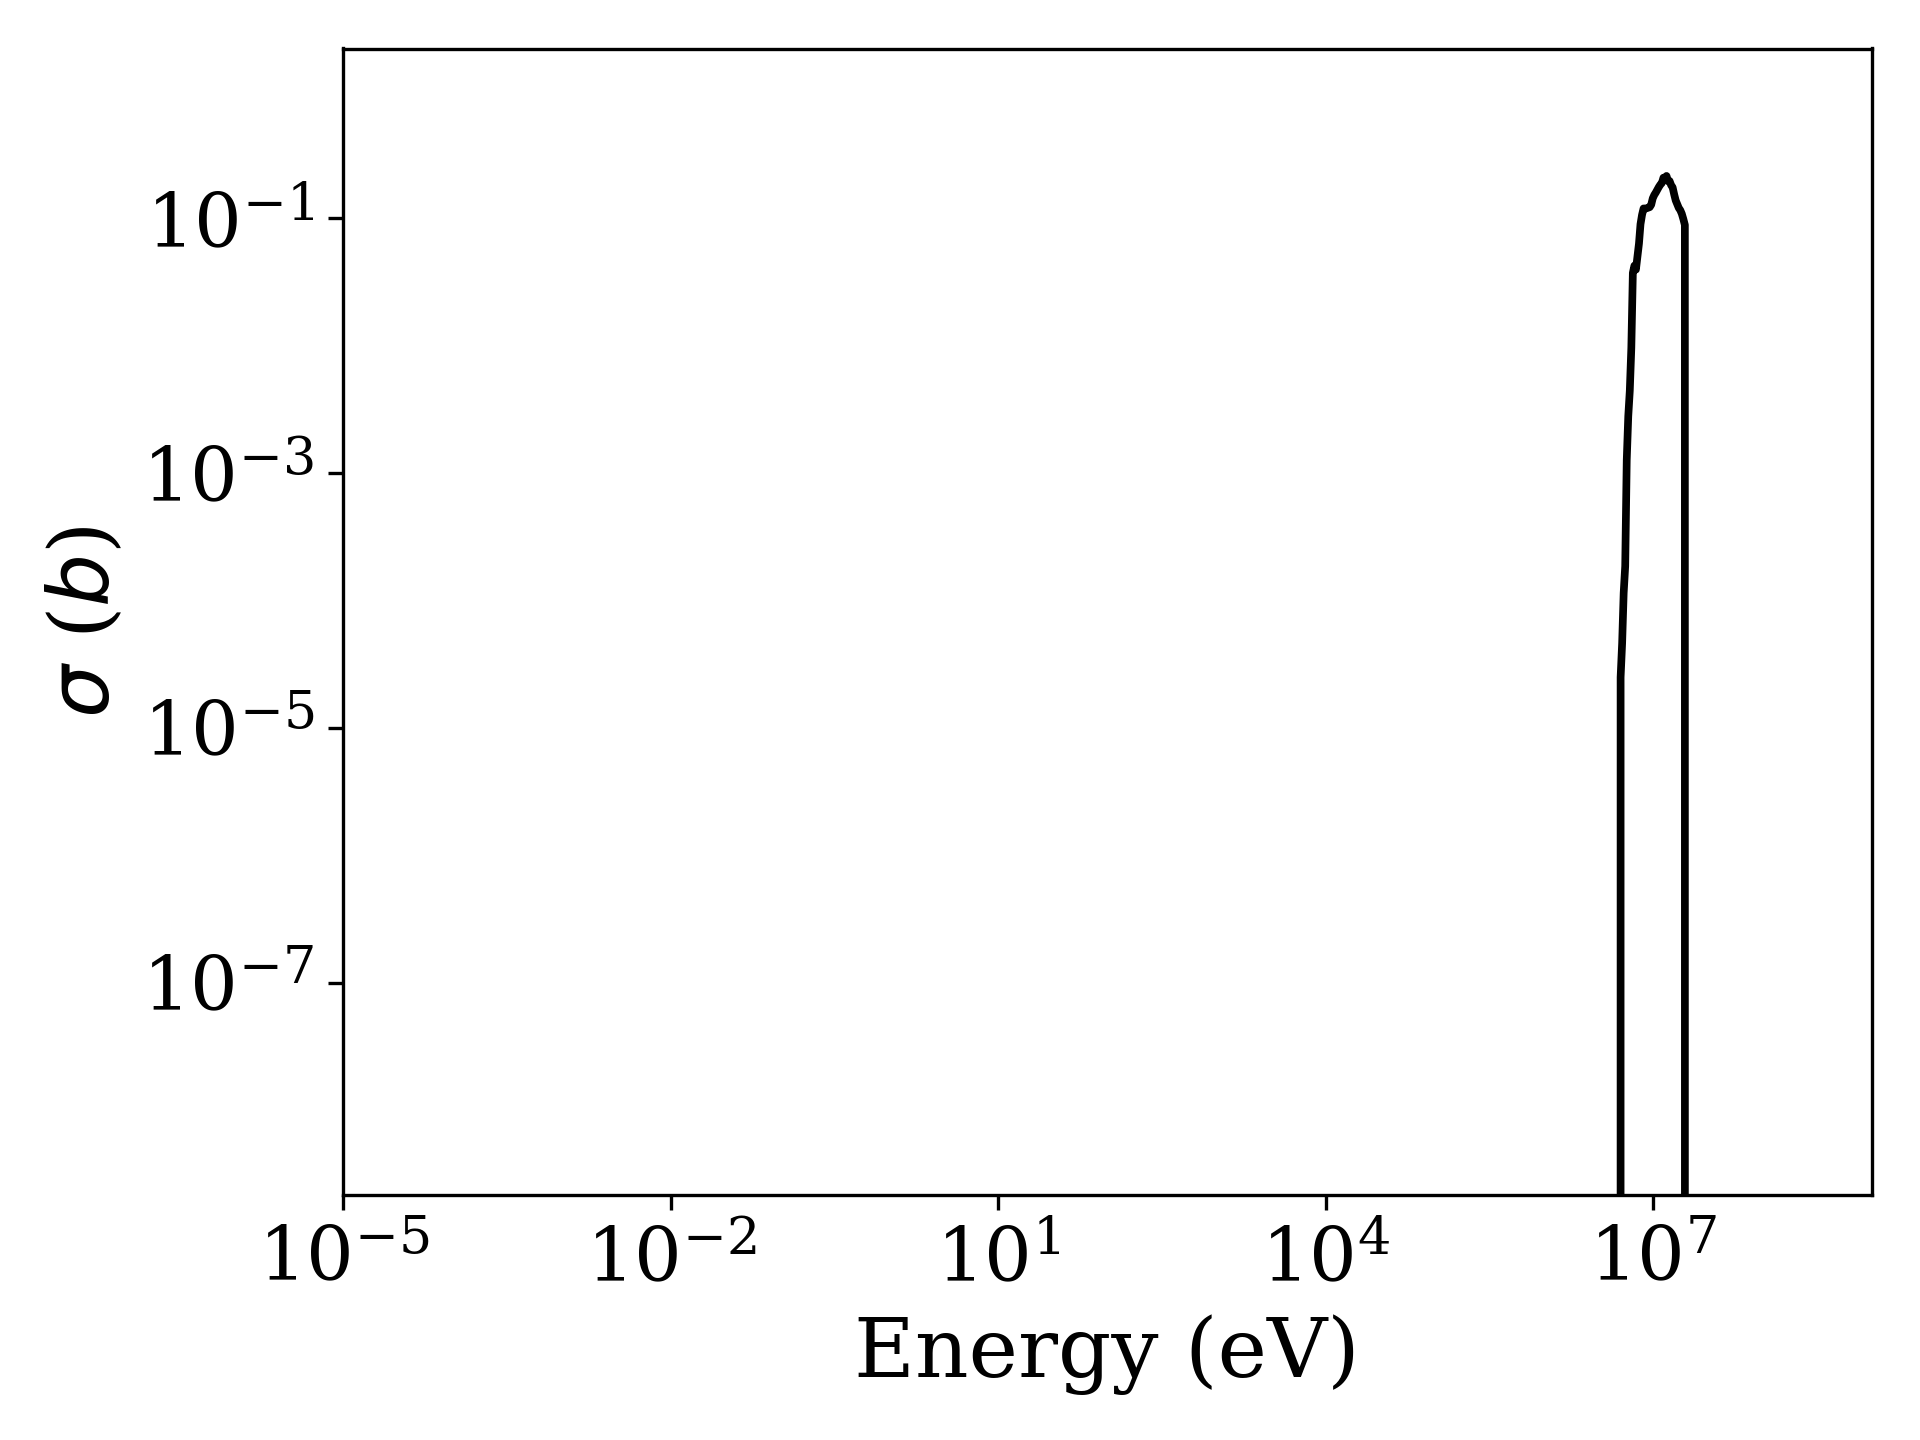
\includegraphics[width=.8\textwidth]{plot/Mg-24(n,p)Na-24} 

  \caption{A subfigure}
  \label{fig:sub2}
\end{subfigure}
\caption{A figure with two subfigures}
\label{fig:test}
\end{figure}

\begin{table*}[h]
\centering
\begin{tabular}{ |c|c|c|c|c|c|c| }
 \hline
 Reaction & T$_{1/2}$ & ROI (eV) & Important Gammas (keV) \\
 \hline 
 $^{24}$Mg(n,p)$^{24}$Na & 15.0 h & 6.46e+06, 1.18e+07 & 1368.626(0.999936) \\ 
\hline
\end{tabular}
\end{table*}
